\lab{Applications}{Wavelet Denoising and Compression}{Denoising and Compression}

\objective{This lab presents applications of the Discrete Wavelet Transform in
image denoising and compression.}

\section*{The PyWavelets Module}
PyWavelets is a Python library for Wavelet Analysis. It provides convenient and
efficient methods to calculate the one and two-dimensional discrete Wavelet
transform, as well as much more. Assuming that the package has been installed on
your machine, type the following to get started:
\begin{lstlisting}
>>> import pywt
\end{lstlisting}
Performing the basic discrete Wavelet transform is very simple.
Below, we compute the one-dimensional transform for a sinusoidal signal.
\begin{lstlisting}
>>> import numpy as np
>>> f = np.sin(np.linspace(0,8*np.pi, 256))
>>> fw = pywt.wavedec(f, 'haar')
\end{lstlisting}
The variable \li{fw} is now a list of arrays, starting with the final approximation
frame, followed by the various levels of detail coefficients, just like the output
of the wavelet transform function that you coded in the previous lab.
Plot the level 2 detail and verify that it resembles a blocky sinusoid.
\begin{lstlisting}
>>> from matplotlib import pyplot as plt
>>> plt.plot(fw[-2], linestyle='steps')
>>> plt.show()
\end{lstlisting}
We can give alter the arguments to the \li{wavedec} function to use different
wavelets or obtain different levels of the wavelet transform. The second
positional argument, as you will notice, is a string that gives the name of the
wavelet to be used. We first used the Haar wavelet, with which you are already
familiar. PyWavelets supports a number of different Wavelets, however, which you can
list by executing the following code:
\begin{lstlisting}
>>> # list the available Wavelet families
>>> print pywt.families()
['haar', 'db', 'sym', 'coif', 'bior', 'rbio', 'dmey']
>>> # list the available wavelets in the coif family
>>> print pywt.wavelist('coif')
['coif1', 'coif2', 'coif3', 'coif4', 'coif5']
\end{lstlisting}
We can also include optional arguments \li{mode} and \li{level} when calling the
\li{wavedec} function. Using these arguments, you can adjust the mode for dealing
with border distortion and the level of the Wavelet decomposition, respectively.

\begin{figure}[t]
    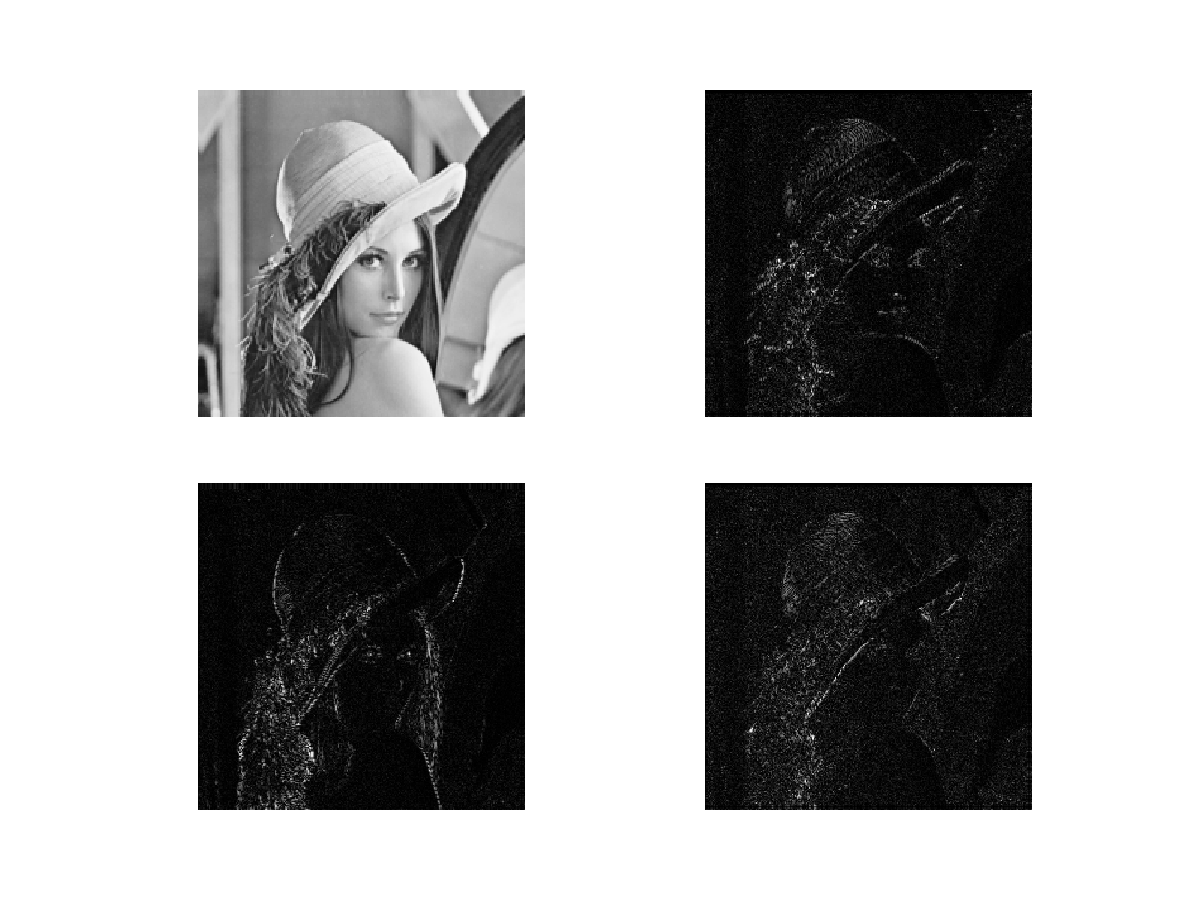
\includegraphics[width=\linewidth]{dwt2.pdf}
    \caption{Level 1 Wavelet decomposition of the Lena image.
    The upper left is the approximation frame, and the remaining
    plots are the detail coefficients.}
    \label{fig:dwt2}
\end{figure}

Now we illustrate how to perform a two-dimensional Wavelet transform using
PyWavelets. We will work with the traditional Lena image, performing a
two level wavelet transform using the Daubechies 4 Wavelet.
\begin{lstlisting}
>>> import scipy.misc
>>> lena = scipy.misc.lena()
>>> lw = pywt.wavedec2(lena, 'db4', level=2)
\end{lstlisting}
The variable \li{lw} is a list of tuples of arrays. The first entry of the list is
simply the level 2 approximation frame. The second entry of the list is a tuple of
the level 2 detail coefficients $LH$, $HL$, and $HH$ (in that order). The remaining
entries of the list are tuples containing the lower level detail coefficients.
Thus, to plot the level 1 $HL$ detail coefficients, we can execute the following code:
\begin{lstlisting}
>>> HL1 = lw[-1][1]
>>> plt.imshow(np.abs(HL1), cmap=plt.cm.Greys_r, interpolation='none')
>>> plt.show()
\end{lstlisting}
The output of this code should be a plot resembling the lower left plot given in Figure
\ref{fig:dwt2}.

We have only introduced a couple of the basic tools available in PyWavelets. There
are of course many more functions and methods that facilitate a more comprehensive
Wavelet analysis. In the remainder of this lab, we will explore three particular 
applications of Wavelet analysis in the realm of image processing and compression.

%\section*{Edge Detection}
%It is often useful to identify the edges of objects and figures
%represented in images. The edge information can be used to classify images
%and group them with other similar images (this is part of a field called
%\textit{computer vision}), to segment the image into component parts, to
%sharpen blurry images, to filter out unnecessary details of the image,
%and so forth. Of course, our human eyes are very adept at recognizing edges,
%but enabling a computer to do the same is much more difficult. An edge can
%be thought of as a discontinuity in the image or a region of high contrast
%in either color or brightness. We can therefore leverage the high-frequency
%detail coefficients of the wavelet transform to detect the edges. Execute the
%following code:
%\begin{lstlisting}
%>>> # calculate one level of wavelet coefficients
%>>> coeffs = pywt.wavedec2(lena,'haar', level=1)
%\end{lstlisting}
%
%Note that the approximation coefficients are very close to the original
%image, while the detail coefficients are much more sparse, and roughly
%capture the edges in the image. In particular, the upper right coefficients
%emphasize the vertical edges, the lower left coefficients emphasize the
%horizontal edges, and the lower right coefficients emphasize the diagonal
%edges.
%
%\begin{problem}
%Now zero out the approximation coefficients and use your inverse DWT
%function to recreate the image. Plot its absolute value. This image is
%a fairly good representation of the edges. If we add this to the original
%image, we can increase the contrast at the edges (that is, make the dark
%side darker, and the light side lighter). Do this, and plot the original
%image side-by-side with the sharpened image. What do you notice? There
%are many image-sharpening techniques, and those based on wavelets
%are more sophisticated than what we have done here, but this gives the
%basic idea.
%\end{problem}
%the above section needs work, or maybe should be taken out completely.

\section*{Noise Removal}
Noise in an image can be defined as unwanted visual artifacts that
obscure the true image. Images can acquire noise from a variety of
sources, including the camera, transmission, and image processing
algorithms. Noise can be completely random and incoherent (as in
Figure \ref{fig:incoherent}), or it can be coherent and display
visual patterns (Figure \ref{fig:coherent}). In this section, we will
focus on reducing a particular type of random noise in images, called
\textit{Gaussian white noise}.

\begin{figure}[t]
\minipage{0.49\textwidth}
    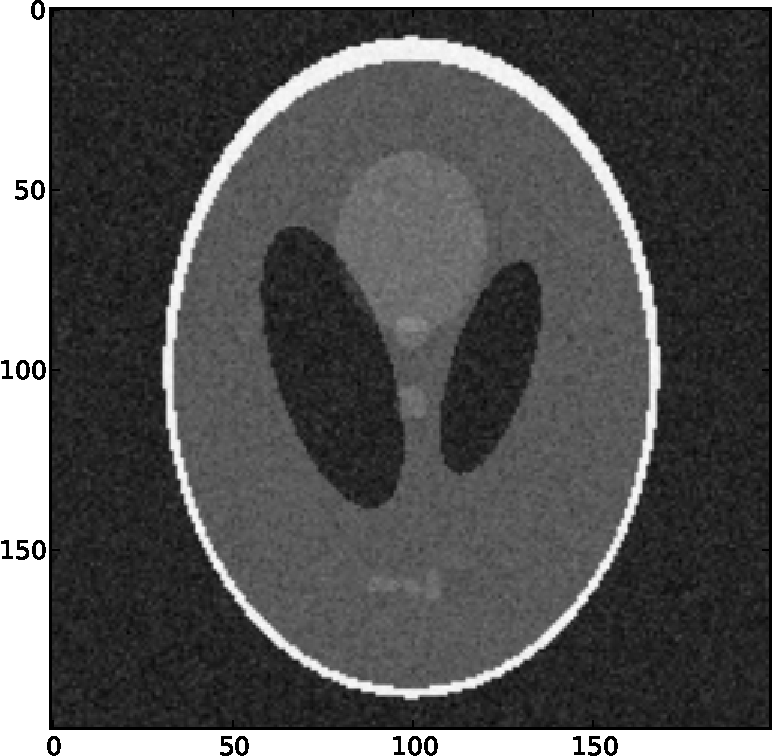
\includegraphics[width=\linewidth]{phantom_random.pdf}
    \caption{The Phantom image with incoherent noise}
    \label{fig:incoherent}
\endminipage\hfill
\minipage{0.49\textwidth}
    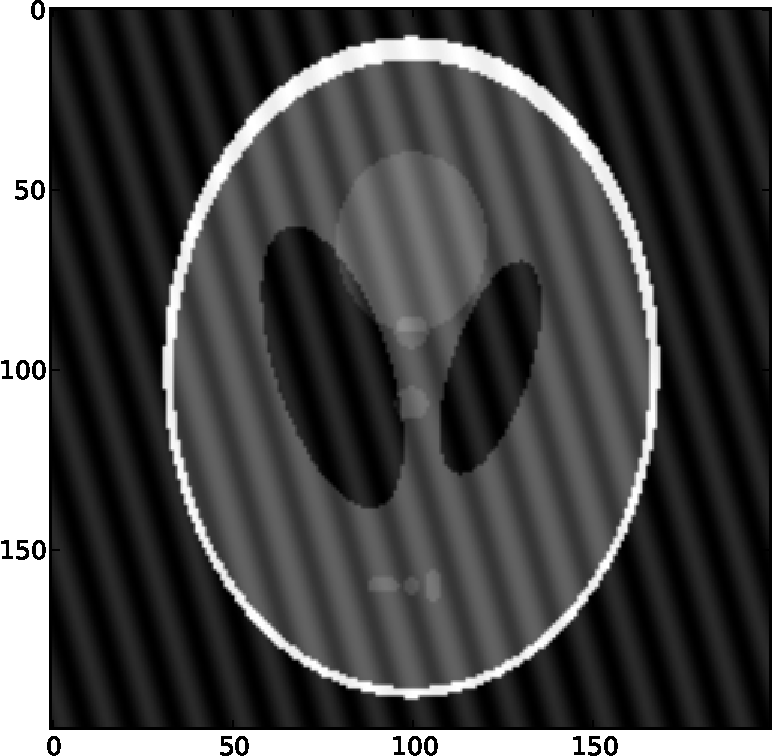
\includegraphics[width=\linewidth]{phantom_coherent.pdf}
    \caption{The Phantom image with coherent noise}
    \label{fig:coherent}
\endminipage
\end{figure}

An image that is distorted by Gaussian white noise is one in which
every pixel has been perturbed by a small amount, such that the
perturbations are normally distributed. We can easily add such noise
to an image using the \li{np.random.normal} function.

\begin{lstlisting}
>>> noisyLena = lena + np.random.normal(scale=20, size=lena.shape)
>>> plt.imshow(noisyLena, cmap=plt.cm.Greys_r)
>>> plt.show()
\end{lstlisting}

Given an image with Gaussian white noise, how do we go about reducing
the noise level? Our approach will be based on the idea of thresholding.
It turns out that images are often sparse in the wavelet basis,
particularly in the high-frequency details. The Gaussian noise, however,
is very high frequency, and thus its wavelet transform will be
concentrated in high-frequency wavelet coefficients (of magnitude
roughly proportional to the variance of the noise). We can therefore
reduce the noise while preserving the true image by shrinking the
detail coefficients via hard or soft thresholding.

Given a positive threshold value $\tau$, hard thresholding sets
every wavelet coefficient whose magnitude is less than $\tau$ to
zero, while leaving the remaining coefficients untouched. Soft
thresholding also zeros out all coefficients of magnitude less than
$\tau$, but in addition maps every other coefficient $\beta$ to
$\beta - \tau$ if $\beta > 0$ or $\beta + \tau$ if $\beta < 0$.

Implementing these simple thresholding algorithms in Python is 
straight-forward, but PyWavelets already provides this functionality.
The following code gives an example.

\begin{lstlisting}
>>> A = np.arange(-4,5).reshape(3,3)
>>> A
array([[-4, -3, -2],
       [-1,  0,  1],
       [ 2,  3,  4]])
>>> pywt.thresholding.hard(A,1.5)
array([[-4, -3, -2],
       [ 0,  0,  0],
       [ 2,  3,  4]])
>>> pywt.thresholding.soft(A,1.5)
array([[-2.5, -1.5, -0.5],
       [ 0. ,  0. ,  0. ],
       [ 0.5,  1.5,  2.5]])
\end{lstlisting}

Once the coefficients have been thresholded, we take the inverse
wavelet transform to recover the denoised image. This can be done
by calling the \li{waverec2} function, providing the list of Wavelet
coefficients as well as the name of the desired Wavelet as arguments.
The threshold value is generally a function of the variance of the noise,
and in real situations, we do not know what this variance is. In fact,
noise variance estimation in images is a research area in its own
right, but this goes beyond the scope of this lab, and so we will
assume that we already have a decent estimate of the variance.

\begin{figure}[t]
    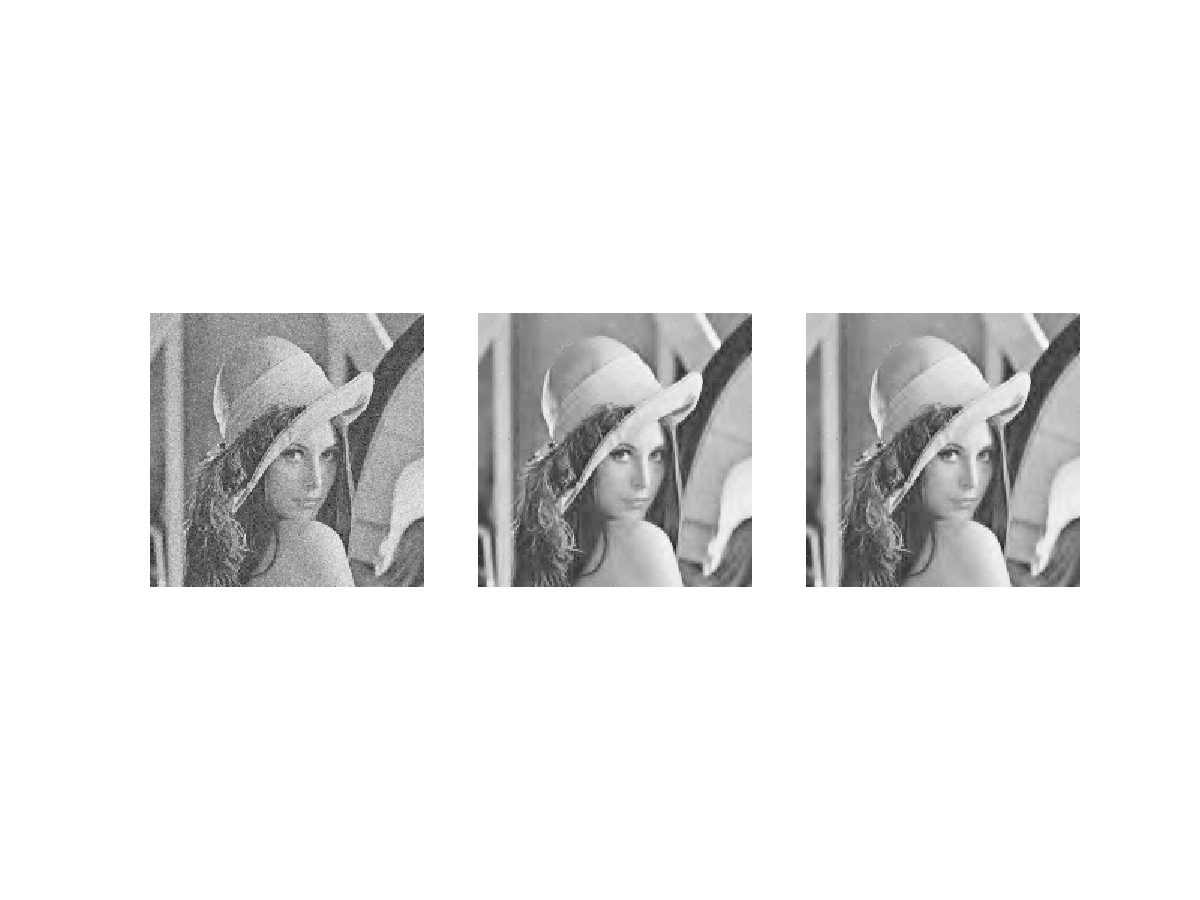
\includegraphics[width=\linewidth]{denoise.pdf}
    \caption{Noisy Lena (left), denoised using hard thresholding (center), 
    and denoised using soft thresholding (right).}
    \label{fig:denoise}
\end{figure}

\begin{problem}
Write functions that implement the hard and soft thresholding
techniques. The inputs should be a list of wavelet coefficients
in the usual form, as well as the threshold value. The output
should be the thresholded wavelet coefficients (also in
the usual form). Remember that we only want to threshold the
detail coefficients, and not the approximation coefficients.
You should therefore leave the first entry of the input
coefficient list unchanged.
\end{problem}

\begin{problem}
Create a noisy version of the Lena image by adding Gaussian
white noise of mean 0 and standard deviation $\sigma = 20$ (i.e. \li{scale=20}).
Compute four levels of the wavelet coefficients using the Daubechies 4 Wavelet, 
and input these into your
thresholding functions (with $\tau = 3\sigma$ for the hard threshold,
and $\tau = 3\sigma/2$ for the soft threshold). Reconstruct the
two denoised images, and then plot these together alongside the
noisy image. Your output should match Figure \ref{fig:denoise}.

What do you notice? How does lowering or raising the
threshold affect the reconstructed images? What happens if you use
a different Wavelet?
\end{problem}

\section*{Image Compression}
We now turn to the problem of image compression. Explicitly saving
the value of every pixel in an image can be very costly in both
storage and transmission, and numerous image compression techniques
have been developed over the years to deal with this problem.
Transform methods have long played an important role in these
techniques; the popular JPEG image compression standard is based on
the discrete cosine transform. Starting from the early 1990's, much
research has gone into compression methods using the discrete wavelet
transform, and to great success. The JPEG2000 compression standard
and the FBI Fingerprint Image database, along with other systems,
take the wavelet approach.

The general framework for compression is fairly straightforward. First,
the image to be compressed undergoes some form of preprocessing (this
can include subtracting out its mean, tiling the image, or perhaps
nothing at all). Next, the wavelet coefficients are computed using some
specially constructed wavelet (JPEG2000 uses the either the
Cohen-Daubechies-Feauveau 9/7 or 5/3 wavelet) and then \textit{quantized},
 a process that we will explain shortly. The quantized coefficients are
 then grouped in a particular way and passed through an entropy encoder
 (such as Huffman coding, run length coding, or arithmetic coding). This
 coding step comes from the realm of information theory, and we will not
 worry about it in this lab. What you have left is a compact stream of bits
 that can then be saved or transmitted much more efficiently than the
 original image. All of the above steps are invertible, allowing us to
 reconstruct the image from the bitstream.

 The step in this process that we will focus on is quantization. Put simply,
 quantization is a process whereby the coefficients are converted into
 integers. If the coefficients are floating-point numbers, then this
 process introduces some loss of precision, and we call this \textit{
 lossy compression}. In the situation where all the coefficients are already
 integers, it is possible to compress the image without any loss of precision,
 and this is called \textit{lossless compression}. Quantization can be
 performed in a variety of ways, and we will explore one particular method
 called a \emph{uniform null-zone quantizer}. Given a coefficient $x$, we assign
 to it an integer $q$ given by
\begin{equation*}
q =
 \begin{cases}
   \lceil x / \delta - t/2 \rceil, &  x \geq 0\\
   \lfloor x / \delta + t/2 \rfloor & x \leq 0
 \end{cases}
\end{equation*}
where $1 \leq t \leq 2$ and $\delta > 0$ are adjustable parameters.
The inverse process, called de-quantization, consists of recovering
the coefficient $y$ from the quantized value $q$ via the equation
\begin{equation*}
 y =
  \begin{cases}
   (q - 1/2 + t/2)\delta & q > 0\\
   (q + 1/2 - t/2)\delta & q < 0\\
   0,                    & q = 0
  \end{cases}
 \end{equation*}
What we are essentially doing is mapping all wavelet coefficients that
fall in the interval $[-\delta,\delta]$ to 0 and all wavelet coefficients
in the interval $[j\delta,(j+1)\delta]$ to $(2j+1)\delta/2$ for integers
$j \geq 1$ and $j \leq -2$. This greatly reduces the number of distinct
coefficient values (indeed, most of the coefficients are mapped to
zero), allowing us, at the cost of some precision, to store less
information. The larger we choose $\delta$, the more compression we
can achieve, albeit with a correspondingly larger loss in precision.
\begin{problem}
Write function \li{quantize} and \li{dequantize} based on the discussion above.
In both cases, the inputs should be a list of wavelet coefficients in
standard form, the $\delta$ parameter, and the $t$ parameter with default
value of 2. The functions should return the quantized list of wavelet
coefficients.

For the Lena image, calculate the complete set of wavelet coefficients and then
quantize and de-quantize the coefficients, and reconstruct the image.
Do this for a few different values of $\delta$ (with $t=2$), and observe how
the image is distorted. Try using different Wavelets. Keep in mind that there are
specially designed Wavelets used in image compression that are not available
in PyWavelets, so distortion will be greater than tolerable in real-life settings.
\end{problem}
